%%
%% This is file `swuthesis-graduate-main.tex',
%% generated with the docstrip utility.
%%
%% The original source files were:
%%
%% swuthesis.dtx  (with options: `graduate')
%% This is a generated file.
%% 
%% It was extracted from swuthesis.dtx.


%%
%% 研究生（博士/硕士）共用示例：与 swuthesis-main.tex（本科）并列，
%% 用于回归测试 |doctor| / |master| 分支。
%% 默认 |master|；若写博士论文，将下面 |\documentclass| 首项改为 |doctor|，
%% 并相应修改 |\swusetup| 中的 |degree| 等字段。
%% 封面论文类型行：主行 |\swuCoverThesisLabelText|（|thesis-label| 或类选项默认）；
%% 可选第二行由 |thesis-label-sub| 写说明文字（不含全角括号），
%% 模板自动加 |（）| 并以一号右圆加粗排出。
%% 英文题名页 |thesis-label-sub-en|：与 |thesis-label-sub| 一项对一行英文（勿写半角括号）；
%% 同等学力、高校教师等\textbf{择一}，译法常见为%
%% |Equivalent Qualification Applicant| / |In-service Faculty Program|；%
%% 中文多项时用 |\par| 与顿号顺序一致。
%% 印刷用纸颜色（规范附件）：博士浅灰；全日制硕士自科浅绿/社科浅黄；%
%% 高校教师与同等学力硕士浅蓝；专业学位博士见附件说明%
%% （印制表格上「打印时此行取消」按学校通知）。本 PDF 不设封面底色。
%% 编译前请在目录 figures/ 下准备 swu-badge.pdf、swu-name-stxingkai.pdf；
%% 若有英文/通用横排校名 swu-name.pdf，置于同目录（可选，类文件会自动叠排）。
%%
\begin{filecontents*}[overwrite]{swuthesis-graduate-main.bib}
@standard{gbt7714,
  title        = {信息与文献 参考文献著录规则},
  organization = {国家市场监督管理总局、
    国家标准化管理委员会},
  number       = {GB/T 7714---2025},
  year         = {2025},
  address      = {北京},
  publisher    = {中国标准出版社}
}

@book{knuth1984texbook,
  author    = {Donald E. Knuth},
  title     = {The {\TeX}book},
  volume    = {A},
  series    = {Computers and Typesetting},
  publisher = {Addison-Wesley},
  year      = {1984},
  address   = {Reading, MA}
}

@book{lamport1994latex,
  author    = {Leslie Lamport},
  title     = {{\LaTeX}: A Document Preparation System},
  edition   = {2},
  publisher = {Addison-Wesley},
  year      = {1994},
  address   = {Reading, MA}
}

@book{mittelbach2004companion,
  author    = {Frank Mittelbach and Michel Goossens and Johannes Braams
    and David Carlisle},
  title     = {The {\LaTeX} Companion},
  edition   = {2},
  publisher = {Addison-Wesley},
  year      = {2004},
  address   = {Boston}
}

@manual{ctex2022,
  title        = {{CTeX} 宏集手册},
  author       = {{CTeX-org}},
  organization = {CTeX-org},
  year         = {2022},
  note         = {CTAN: https://ctan.org/pkg/ctex. 引用日期: 2026-04-18.},
  langid       = {chinese}
}

@book{zhouzhihua2016ml,
  author    = {周志华},
  title     = {机器学习},
  publisher = {清华大学出版社},
  year      = {2016},
  address   = {北京},
  isbn      = {978-7-302-42328-7},
  langid    = {chinese}
}

@article{liguojie2012bigdata,
  author       = {李国杰 and 程学旗},
  title        = {大数据研究: 未来科技及经济社会发展的重大战略领域——
    大数据的研究现状与科学思考},
  journaltitle = {中国科学院院刊},
  year         = {2012},
  volume       = {27},
  number       = {6},
  pages        = {647--657},
  issn         = {1000-3045},
  langid       = {chinese}
}

@article{WalpuskiZhang2021DMJ,
  author       = {Walpuski, Thomas and Zhang, Boyu},
  title        = {On the Compactness Problem for a Family of Generalized
    {Seiberg--Witten} Equations in Dimension 3},
  journaltitle = {Duke Mathematical Journal},
  shortjournal = {Duke Math. J.},
  volume       = {170},
  number       = {17},
  pages        = {3891--3934},
  year         = {2021},
  doi          = {10.1215/00127094-2021-0005},
  note         = {MathSciNet MR4340726},
  langid       = {english}
}

@misc{taubes2020compactness,
  author     = {Taubes, Clifford Henry},
  title      = {{Compactness for $\mathrm{SL}(2;\mathbb{C})$ and 4D anti-self dual
    equations}},
  year       = {2020},
  eprinttype = {arxiv},
  eprint     = {1307.6447},
  langid     = {english}
}

@inproceedings{vaswani2017attention,
  author    = {Vaswani, Ashish and Shazeer, Noam and Parmar, Niki and Uszkoreit, Jakob
    and Jones, Llion and Gomez, Aidan N. and Kaiser, {\L}ukasz and Polosukhin, Illia},
  title     = {Attention Is All You Need},
  booktitle = {Advances in Neural Information Processing Systems 30:
    Proceedings of the 31st Conference on Neural Information Processing Systems},
  year      = {2017},
  pages     = {5998--6008},
  publisher = {Curran Associates, Inc.},
  address   = {Long Beach, CA, USA},
  langid    = {english}
}

@online{swu2022gradThesisSpecDoc,
  author    = {{西南大学}},
  title     = {西南大学博士硕士学位论文规范},
  date      = {2022-06-28},
  url       = {https://dwyx.swu.edu.cn/info/1083/2038.htm},
  urldate   = {2026-04-18},
  note      = {西南大学博士硕士学位论文规范.doc},
  langid    = {chinese}
}

@online{swu2021thesisManageNotice,
  author    = {{西南大学}},
  title     = {关于印发《西南大学全日制本科学生毕业论文（设计）工作管理办法》的通知},
  date      = {2021-01-07},
  url       = {https://ceie.swu.edu.cn/info/1125/3918.htm},
  urldate   = {2026-04-18},
  note      = {西校〔2021〕4号},
  langid    = {chinese}
}

@online{swuUndergradThesisSpecWeb,
  author    = {{西南大学}},
  title     = {西南大学本科毕业论文（设计）规范},
  url       = {https://ceie.swu.edu.cn/info/1125/3918.htm},
  urldate   = {2026-04-18},
  note      = {门户亦可能发布 \texttt{.docx} 直链；以当期页面为准。},
  langid    = {chinese}
}

@misc{bao2024swuthesisLegacy,
  author       = {包小敏},
  title        = {西南大学本科毕业论文 {\LaTeX} 模板（本科毕业论文模板\_新）},
  year         = {2024},
  month        = aug,
  howpublished = {西南大学数学与统计学院本科毕业论文写作模板；含 myTemplate.tex、SWUthesis.sty 等},
  note         = {持续维护至 2024 年；联系信箱 xbao@swu.edu.cn},
  langid       = {chinese}
}
\end{filecontents*}

\documentclass[master,fontset=macnew,punct=banjiao]{swuthesis}

\usepackage{subcaption}
\usepackage{longtable}
\usepackage{siunitx}
\usepackage{tikz}
\usetikzlibrary{arrows.meta,positioning}
\sisetup{detect-all}

\swusetup{
  title          = {西南大学\swuThesisTierZh 学位论文模板示例},
  subtitle       = {可选副标题},
  title-en       = {An Example Thesis for Southwest University},
  college        = {数学与统计学院},
  college-en     = {School of Mathematics and Statistics},
  major          = {基础数学},
  research-field = {微分几何与拓扑},
  author         = {张三},
  author-en      = {San Zhang},
  student-id     = {12020101000001},
  supervisor     = {李四\ 教授},
  supervisor-en  = {Prof.\ Si Li},
  submitted-school-en = {Graduate School},
  university-en       = {Southwest University},
  graduate-program-en = {Graduate Program in School of Mathematics and Statistics},
  degree         = {理学硕士},
  degree-en      = {Master of Science in Mathematics},
  defense-location-en = {Chongqing, P.R. China},
  submit-date    = {2026/3/15},
  defense-date   = {2026/6/18},
  %thesis-label     = {硕士学位论文},
  %thesis-label-sub    = {高校教师},
  %thesis-label-sub-en = {In-service Faculty Program},
  % 同等学力论文请改为：thesis-label-sub = {同等学力},
  % thesis-label-sub-en = {Equivalent Qualification Applicant},
}

\addbibresource{swuthesis-graduate-main.bib}

\begin{document}

\frontmatter
\maketitle
\tableofcontents

\begin{cnabstract}
本文给出面向西南大学\swuThesisTierZh 学位论文的 \LaTeX{} 模板示例文档，%
与本科示例 \path{swuthesis-main.tex} 功能对齐：%
演示研究生规范式封面与中英文题名页、摘要生成、章节结构、插图与子图、三线表与长表格、数学公式与交叉引用、%
定理类环境、GB/T~7714 参考文献著录、致谢与在读期间科研成果，%
以及附录中《西南大学本科毕业论文（设计）规范》%
全文与多语言 \texttt{listings} 代码示例（与本科示例同源，便于对照）。%
撰写与提交时请以《西南大学博士硕士学位论文规范》%
及学院最新通知为准；本文件侧重版式与工具链说明，不能替代对选题与学术规范的理解。
\end{cnabstract}
\begin{cnkeywords}
西南大学；\swuThesisTierZh 学位论文；\LaTeX；模板示例；排版
\end{cnkeywords}
\begin{enabstract}
This document is a \swuThesisEnDocRole{} example for Southwest University,%
parallel in scope to the undergraduate \texttt{swuthesis-main.tex}.%
It demonstrates the graduate cover and English title page, bilingual abstract,%
chapter organization, figures and subfigures,%
three-line and long tables, numbered equations and cross-references,%
theorem-like environments, bibliography formatting, acknowledgements (\texttt{ack}),%
and publications during the degree.%
Like \texttt{swuthesis-main.tex}, the appendix includes%
the full undergraduate thesis specification text and%
multi-language \texttt{listings} examples for regression testing.%
Formal requirements follow the university's doctoral and master's thesis specification;%
this file focuses on typesetting and the tool chain.
\end{enabstract}
\begin{enkeywords}
Southwest University; \swuThesisEnDocRole; \LaTeX; template example; typesetting
\end{enkeywords}
\makeabstract

\mainmatter
\chapter{模板与规范说明}\label{ch:doctor-guide}

本章说明本研究生示例文档的用途，以及模板与学校正式规范之间的关系。%
\swuThesisTierZh 学位论文的撰写、结构与排版以《西南大学博士硕士学位论文规范》为准%
\cite{swu2022gradThesisSpecDoc}%
（学校页面提供 \texttt{.doc} 下载，以学校及学院最新发布为准）。%
本科毕业论文（设计）另有《西南大学全日制本科学生毕业论文（设计）工作管理办法》（西校〔2021〕4号）及%
《西南大学本科毕业论文（设计）规范》等文件%
\cite{swu2021thesisManageNotice,swuUndergradThesisSpecWeb}。%
\textbf{为与本科示例 \path{swuthesis-main.tex} 回归测试对齐，该本科规范的完整条文仍收录于附录~\ref{app:swu-undergrad-spec}}；
研究生正式写作请以研究生规范为准，勿将本科附录条文误作\swuThesisTierZh 学位论文要求。
旧版以 \path{SWUthesis.sty} 等组织的模板在工作流程上仍有参考价值%
\cite{bao2024swuthesisLegacy}；%
本仓库 \texttt{swuthesis} 为基于 \path{swuthesis.dtx} 的文档类实现，%
便于本科、硕士、博士分支统一维护。

\section{编译与工具链}\label{sec:doctor-compile}
\subsection{引擎与参考文献后端}
\begingroup\sloppy
正文为中文并依赖字体与 \texttt{ctex}，\textbf{须使用 \hologo{XeLaTeX}} 编译。
参考文献使用 \texttt{biblatex}，\textbf{须运行 \hologo{biber}}（随 TeX~Live、MiKTeX 等发行版安装；在编辑器中将「参考文献处理器」设为 \hologo{biber}）。
\textbf{不要使用}以 \hologo{pdfLaTeX} 为默认的一键流程（例如 WinEdt 中常见的 PDF\TeX{}ify），否则无法正确排版中文与参考文献。
\par\endgroup

\subsection{Windows（含 WinEdt）}
\begin{itemize}
  \item \textbf{Biber 与 WinEdt}：在 \texttt{TeX} $\rightarrow$ \texttt{Execution Modes}%
    （或同类菜单）中，将主流程设为 \textbf{\hologo{XeLaTeX}}，%
    并在需要时增加一步 \hologo{biber}，再多次 \hologo{XeLaTeX}，%
    顺序与下文 \cref{sec:doctor-compile-make} 一致即可。
  \item \textbf{避免 PDF\TeX{}ify}：该快捷方式通常绑定 \hologo{pdfLaTeX}，与本模板不兼容。
  \item 若已安装 TeX~Live 并将 \texttt{bin} 加入系统 \texttt{PATH}，%
    也可在「命令提示符」或 PowerShell 中进入工程目录，%
    手动执行与 \cref{sec:doctor-compile-make} 相同的命令。
\end{itemize}

\subsection{macOS / Linux 与 \texttt{Makefile}}\label{sec:doctor-compile-make}
工程根目录的 \path{Makefile} 目标 \texttt{graduate} 会依次执行：
\hologo{XeLaTeX} $\rightarrow$ \hologo{biber} $\rightarrow$ \hologo{XeLaTeX}%
  $\rightarrow$ \hologo{XeLaTeX}。
在终端进入工程目录后执行 \texttt{make graduate} 即可。%
\textbf{\texttt{make}} 为系统自带或随「构建工具」安装：%
macOS 若提示无此命令，可安装 Xcode Command Line Tools；%
执行 \texttt{xcode-select --install}。%
Linux 可通过包管理器安装 \texttt{make} 或 \texttt{build-essential}。%
Windows 可使用 MSYS2、Git for Windows 环境，或 WSL 中的 GNU \texttt{make}。%

\subsection{持续编译（\texttt{latexmk}）}
TeX~Live 等发行版自带 \texttt{latexmk}，可根据辅助文件自动决定运行次数及是否调用 \hologo{biber}。写作时可在工程目录使用：
\begin{verbatim}
latexmk -pvc -xelatex swuthesis-graduate-main.tex
\end{verbatim}
选项 \texttt{-pvc} 表示持续预览。%
若工程根目录提供 \path{.latexmkrc}（本仓库已含），亦可简写为%
\texttt{latexmk -pvc} \texttt{swuthesis-graduate-main.tex}。%
首次编译前请已生成 \path{swuthesis.cls}%
（例如 \texttt{latex swuthesis.ins} 或 \texttt{make cls}）。%

\subsection{编译质量检查（含 Overfull/Underfull）}\label{sec:doctor-compile-quality-check}
研究生论文常包含长表格、公式与双语字段，建议每次完整编译后检查日志。
命令 \texttt{rg} 为 \textbf{ripgrep}，须单独安装（\TeX{} Live 不自带）；%
macOS 常用 \texttt{brew install ripgrep}，%
Windows 可用 \texttt{winget install BurntSushi.ripgrep}，%
Linux 可用发行版包管理器安装。%
若未安装 \texttt{rg}，可改用 \texttt{grep}，例如%
\texttt{grep Overfull swuthesis-graduate-main.log} 等。
\begin{verbatim}
rg Overfull swuthesis-graduate-main.log
rg Underfull swuthesis-graduate-main.log
rg "Missing character" swuthesis-graduate-main.log
\end{verbatim}
处理原则与 \cref{sec:compile-quality-check} 一致：优先修正 \texttt{Overfull} 与%
\texttt{Missing character}，%
对 \texttt{Underfull} 结合版式位置与可读性判断。若需汇总检查全部示例，可在 \texttt{make all} 后执行：
\begin{verbatim}
rg Overfull *.log
rg Underfull *.log
rg "Missing character" *.log
\end{verbatim}

\section{与既有本科毕业论文模板的关系及本模板的必要性}
西南大学本科论文写作中长期流传着一类以 \textsf{ctexbook} 为主文档类、%
以 \path{SWUthesis.sty} 为版式与宏包集合、%
用 \texttt{\textbackslash include} 分文件组织封面、声明、摘要与正文的模板%
（坊间多称「本科毕业论文模板\_新」等；可参考文献\cite{bao2024swuthesisLegacy}）。
其在\textbf{工作流程}与\textbf{版式目标}上为本项目提供了\textbf{部分经验参考}。%
本仓库 \texttt{swuthesis} 并非在上述 \texttt{.sty} 源码上逐行修补，%
而是\textbf{全新设计}的文档类：以 \path{swuthesis.dtx} 生成 \path{swuthesis.cls}，%
用 \LaTeX3 键值接口集中论文元信息，参考文献采用 \texttt{biblatex} 与 GB/T~7714 系列样式。%
这样做的必要性在于：
\begin{enumerate}[label=\arabic*., leftmargin=2em]
  \item \textbf{可维护性与可重复构建}：单一类文件 + 主文档，版本信息清晰，便于随学校规范修订而更新。
  \item \textbf{与现代工具链一致}：与当前 \TeX{} Live 生态对齐，降低在新系统上的故障率。
  \item \textbf{扩展空间}：同一套类文件覆盖本科、硕士、博士，减少多套工程重复同步版式。
\end{enumerate}

\section{示例文档的定位}
\texttt{swuthesis-graduate-main.tex} 用于检验 \texttt{doctor} / \texttt{master} 选项下封面（含英文题名页）、%
摘要、目录、章节、图表、公式、定理环境、参考文献、致谢、%
\texttt{publications} 环境及附录等能否正确生成。%
\LaTeX{} 负责版式与自动化，\textbf{不能替代}对研究问题、方法与学术诚信的把握。

\section{与学校规范的关系}
学校对研究生学位论文字数、结构、参考文献、装袋材料等有统一要求。%
正文各章演示排版命令的用法；%
\textbf{研究生条文级要求}以《西南大学博士硕士学位论文规范》%
\cite{swu2022gradThesisSpecDoc} 为准。%
\textbf{本科规范全文}仅附录~\ref{app:swu-undergrad-spec} 用于对照本科示例与 \texttt{listings} 回归测试。%
学院若有补充规定，以学院通知为准。

\section{阅读与修改建议}
撰写真实\swuThesisTierZh 学位论文时，建议先通读研究生院发布的最新规范，%
再按学院模板整理材料；使用本模板时，可在导言区按需载入宏包，%
但不宜改动学校规定的封面与声明页要素。

\section{程序代码与 \texttt{listings}}\label{sec:doctor-code}
\texttt{swuthesis} 已载入 \texttt{listings} 并定义代码样式。%
正文中可使用 \texttt{\textbackslash lstinline}、\texttt{lstlisting} 环境或%
\texttt{\textbackslash lstinputlisting} 从子目录引入源码。%
Matlab、Wolfram 语言（\texttt{listings} 中标识为 \texttt{Mathematica}）、Python、R、C++ 等示例见附录~\ref{app:code-matlab}--\ref{app:code-cpp}。

\paragraph{附录示例来源说明}
文末附录设有标题为\textbf{附录示例来源说明}的一节（见\hyperref[app:source-note]{该处}），说明程序附录与先行模板及文献\cite{bao2024swuthesisLegacy} 之间的关系。正式撰写时，若使用或改写示例代码，建议在致谢或说明中予以交代。

\chapter{插图}\label{ch:doctor-figures}

\section{使用 \texttt{graphicx} 插入外部图片}
\begingroup\sloppy
以下使用 \TeX~Live 等发行版自带的示例图（\textsf{mwe} 宏包中的 \texttt{example-image-a}、\texttt{example-image-b} 与 \texttt{example-image-c}）。
这些资源随发行版安装，无需复制到工程目录即可编译；实际写作时替换为自有文件即可。
\par\endgroup

\subsection{单幅图}
\begin{figure}[htbp]
  \centering
  \includegraphics[width=0.55\textwidth]{example-image-a}
  \caption{单幅插图示例（\swuThesisTierZh 学位论文示例，\texttt{example-image-a}）}
  \label{fig:doctor-graphicx-single}
\end{figure}

\subsection{左右子图}
\begin{figure}[htbp]
  \centering
  \begin{subfigure}[b]{0.47\textwidth}
    \centering
    \includegraphics[width=\linewidth]{example-image-b}
    \caption{左侧子图}
    \label{fig:doctor-sub-left}
  \end{subfigure}
  \hfill
  \begin{subfigure}[b]{0.47\textwidth}
    \centering
    \includegraphics[width=\linewidth]{example-image-c}
    \caption{右侧子图}
    \label{fig:doctor-sub-right}
  \end{subfigure}
  \caption{左右子图排版示例}
  \label{fig:doctor-subfigures}
\end{figure}

由 \cref{fig:doctor-graphicx-single,fig:doctor-subfigures} 可见，图题置于图下方；子图可采用 \texttt{[b]} 底部对齐。

\section{TikZ 绘图示例}
\begin{figure}[htbp]
  \centering
  \begin{tikzpicture}[node distance=18mm,>=Latex]
    \node[draw,rounded corners,minimum width=28mm,minimum height=10mm] (spec) {学位规范};
    \node[draw,rounded corners,right=of spec,%
      minimum width=28mm,minimum height=10mm] (class) {\texttt{swuthesis}};
    \node[draw,rounded corners,right=of class,%
      minimum width=28mm,minimum height=10mm] (main) {主文档};
    \draw[->,thick] (spec) -- (class);
    \draw[->,thick] (class) -- (main);
  \end{tikzpicture}
  \caption{规范—类文件—主文档关系示意图（TikZ）}
  \label{fig:doctor-tikz-workflow}
\end{figure}

\subsection{并列示意子图}
\begin{figure}[htbp]
  \centering
  \begin{subfigure}[b]{0.47\textwidth}
    \centering
    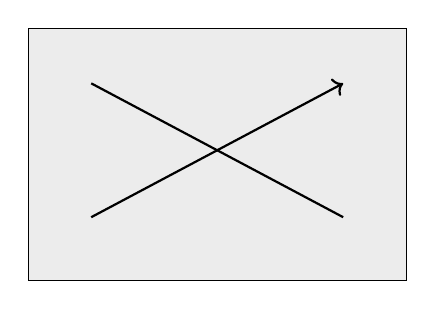
\begin{tikzpicture}
      \draw[fill=gray!15] (0,0) rectangle (4.8,3.2);
      \draw[thick,->] (0.8,0.8) -- (4,2.5);
      \draw[thick] (0.8,2.5) -- (4,0.8);
    \end{tikzpicture}
    \caption{简单示意子图}
    \label{fig:doctor-tikz-sub-left}
  \end{subfigure}
  \hfill
  \begin{subfigure}[b]{0.47\textwidth}
    \centering
    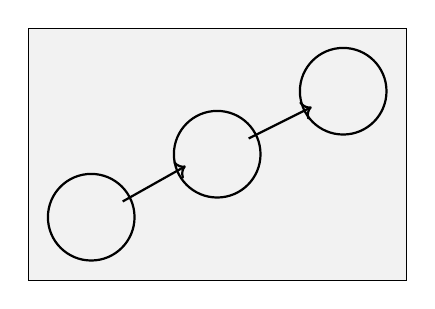
\begin{tikzpicture}
      \draw[fill=gray!10] (0,0) rectangle (4.8,3.2);
      \draw[thick] (0.8,0.8) circle [radius=0.55];
      \draw[thick] (2.4,1.6) circle [radius=0.55];
      \draw[thick] (4.0,2.4) circle [radius=0.55];
      \draw[thick,->] (1.2,1.0) -- (2.0,1.45);
      \draw[thick,->] (2.8,1.8) -- (3.6,2.2);
    \end{tikzpicture}
    \caption{并列对齐子图}
    \label{fig:doctor-tikz-sub-right}
  \end{subfigure}
  \caption{左右两个子图排版示例（TikZ）}
  \label{fig:doctor-tikz-subfigures}
\end{figure}

\cref{fig:doctor-tikz-workflow,fig:doctor-tikz-subfigures} 与上文 \texttt{graphicx} 示例的版式要求一致：图题在图下、子图可对齐引用。

\chapter{表格}\label{ch:doctor-tables}

\section{三线表示例}
\begin{table}[htbp]
  \centering
  \caption{研究生示例中常用环境与用途}
  \label{tab:doctor-booktabs}
  \begin{tabular}{lll}
    \toprule
    环境或命令 & 主要用途 & 备注 \\
    \midrule
    \texttt{\textbackslash chapter} & 一级结构组织 & 按章编号 \\
    \texttt{figure} / \texttt{subfigure} & 插图、子图 & 图题置底 \\
    \texttt{table} / \texttt{longtable} & 表格、跨页表 & 表题置顶 \\
    \texttt{equation} / \texttt{align} & 公式 & 可交叉引用 \\
    \texttt{theorem} 等 & 定理类陈述 & 按章编号 \\
    \bottomrule
  \end{tabular}
\end{table}

\section{数值与 \texttt{siunitx}（示意）}
导言区已 \texttt{\textbackslash usepackage\{siunitx\}} 并%
\texttt{\textbackslash sisetup\{detect-all\}}，%
便于物理量与小数列对齐（与本科示例一致）。%
\begin{table}[htbp]
  \centering
  \caption{\texttt{siunitx} 的 \texttt{S} 列对齐示例}
  \label{tab:doctor-siunitx}
  \begin{tabular}{S[table-format=3.2] S[table-format=2.1]}
    \toprule
    {\heiti 列甲 / m} & {\heiti 列乙 / s} \\
    \midrule
    12.34 & 1.2 \\
    0.88  & 10.0 \\
    \bottomrule
  \end{tabular}
\end{table}

\section{长表格示例}
\begin{longtable}{@{}clp{0.485\textwidth}@{}}
  \caption{\swuThesisTierZh 学位论文常见组成部分（示意，以学校最新规范为准）}\\
  \toprule
  序号 & 部分 & 说明 \\
  \midrule
  \endfirsthead
  \caption[]{\swuThesisTierZh 学位论文常见组成部分（续）}\\
  \toprule
  序号 & 部分 & 说明 \\
  \midrule
  \endhead
  \bottomrule
  \endfoot
  1 & 封面与中英文题名页 & 体现题目、作者、导师、专业、研究方向及提交/答辩日期等。 \\
  2 & 独创性声明与版权使用授权书 & 按学校格式签署。 \\
  3 & 目录 & 一般列到二级标题；页码与正文区分编排方式按规范执行。 \\
  4 & 中英文摘要 & 摘要篇幅、关键词数量等按《博士硕士学位论文规范》执行。 \\
  5 & 正文 & 绪论、各章主体、结论等；可分多章展开研究工作。 \\
  6 & 参考文献 & 著录格式与顺序按 GB/T~7714 及学校要求。 \\
  7 & 致谢 & 致谢对象与范围按学校规定。 \\
  8 & 在读期间取得的科研成果 & 已发表论文、专利、会议论文、科研项目等；致谢之后、附录之前。 \\
  9 & 附录 & 补充材料、符号表、程序等，非必须。 \\
\end{longtable}

\chapter{数学公式}\label{ch:doctor-math}

\section{编号与对齐}
\begin{equation}
  J(\boldsymbol{\beta})=\lVert \mathbf{y}-\mathbf{X}\boldsymbol{\beta} \rVert_2^2.
  \label{eq:doctor-objective}
\end{equation}
\begin{align}
  \frac{\partial J}{\partial \boldsymbol{\beta}}
  &= -2\mathbf{X}^{\mathsf T}\left(\mathbf{y}-\mathbf{X}\boldsymbol{\beta}\right)=0,%
  \label{eq:doctor-gradient}\\
  \mathbf{X}^{\mathsf T}\mathbf{X}\boldsymbol{\beta}
  &= \mathbf{X}^{\mathsf T}\mathbf{y}. \label{eq:doctor-normal}
\end{align}
由 \cref{eq:doctor-objective,eq:doctor-gradient,eq:doctor-normal} 可见编号与 \texttt{\textbackslash cref} 引用正常。

\section{常见符号示例}
下列公式展示了常见的集合、极限、求和、积分和矩阵写法：
\begin{equation}
  A=\left\{x\in\mathbb{R}: x^2\le 1\right\}, \qquad
  \lim_{n\to\infty}\sum_{k=1}^{n}\frac{1}{k^2}=\frac{\pi^2}{6}.
\end{equation}
\begin{equation}
  \int_{0}^{1} x^\alpha (1-x)^\beta\,\mathrm{d}x
  = \frac{\Gamma(\alpha+1)\Gamma(\beta+1)}{\Gamma(\alpha+\beta+2)}.
\end{equation}
\begin{equation}
  \mathbf{A}=
  \begin{bmatrix}
    1 & 0 & 2 \\
    0 & 1 & 3 \\
    2 & 3 & 5
  \end{bmatrix}.
\end{equation}

考虑方程组
\begin{equation}\label{eq:doctor-uniform}
\begin{aligned}
  a\cos\theta+b\sin\theta&=10,\\
  b\cos\theta+a\sin\theta&=10
\end{aligned}
  \implies a^2+b^2=100.
\end{equation}
\eqref{eq:doctor-uniform} 演示了 \texttt{aligned} 置于 \texttt{equation} 内的统一编号。

\section{分段函数与方程组}
分段函数可用 \texttt{cases} 环境排版；例如
\[
  f(\theta):=
  \begin{cases}
    a\cos\theta,&\theta\in[\pi,2\pi),\\
    b\sin\theta,&\theta\in[0,\pi).
  \end{cases}
\]

\chapter{定理环境}\label{ch:doctor-theorem}

\section{定理、定义与证明}

\begin{defn}\label{def:doctor-convex}
若对任意 $x,y\in \mathbb{R}^n$ 和任意 $\lambda\in[0,1]$，都有
$f(\lambda x+(1-\lambda)y)\le \lambda f(x)+(1-\lambda)f(y)$，则称 $f$ 为凸函数。
\end{defn}

\begin{thm}[Jensen不等式]\label{thm:doctor-jensen}
设 $f$ 是区间 $I$ 上的凸函数，$x_1,\dots,x_n\in I$，
$\lambda_1,\dots,\lambda_n\ge 0$ 且 $\sum_{i=1}^{n}\lambda_i=1$，则
$f\!\left(\sum_{i=1}^{n}\lambda_i x_i\right)\le \sum_{i=1}^{n}\lambda_i f(x_i)$。
\end{thm}

\begin{proof}
这是 Jensen 不等式的标准表述。对于离散情形，可由凸函数定义反复应用归纳得到。
\end{proof}

\begin{cor}\label{cor:doctor-amgm}
对任意正数 $a_1,\dots,a_n$，有
\[
\frac{a_1+\cdots+a_n}{n}\ge \sqrt[n]{a_1\cdots a_n}.
\]
\end{cor}

\begin{rmk}
在模板中，\texttt{thm}、\texttt{defn}、\texttt{cor} 等缩写环境与全称%
（\texttt{theorem}、\texttt{definition}、\texttt{corollary} 等）共享计数器，按章编号，%
并可通过 \texttt{\textbackslash cref} 直接引用，%
如 \cref{def:doctor-convex,thm:doctor-jensen,cor:doctor-amgm}。%
\end{rmk}

\chapter{参考文献引用示例}\label{ch:doctor-bib}

\noindent 本示例的%
\path{swuthesis-graduate-main.bib}%
由主文件内 \texttt{filecontents*} 环境生成；%
条目著录与公开书目一致，%
类型涵盖 GB/T~国标、西文专著、\texttt{CTeX} 手册、中文专著与期刊（可在 CNKI 等检索）、%
MathSciNet 著录的数学期刊论文、arXiv 预印本与 NeurIPS 会议论文、%
学校发布的本科与研究生规范网页等；%
键名与本科示例 \path{swuthesis-main.bib} 中部分条目对齐，便于对照维护。%

\section{正文中的引用}
{\sloppy
学术写作中，正文引用应与文后参考文献表一致。使用 \texttt{biblatex} 配合
GB/T~7714 顺序编码样式后，可在正文中混合著录西文专著%
\cite{knuth1984texbook,lamport1994latex,mittelbach2004companion}、%
中文专著（如可在 CNKI 检索的教材）\cite{zhouzhihua2016ml}、%
中文期刊论文\cite{liguojie2012bigdata}、%
英文数学期刊（可在 MathSciNet 按 MR 号或 DOI 核对）\cite{WalpuskiZhang2021DMJ}、%
arXiv 预印本\cite{taubes2020compactness}、会议论文\cite{vaswani2017attention}。%
排版工具说明见 \cite{ctex2022}，著录格式见国家标准 \cite{gbt7714}。%
学校本科与研究生管理文件见 \cite{swu2021thesisManageNotice,swuUndergradThesisSpecWeb,%
swu2022gradThesisSpecDoc}。%
\par}

\section{文后文献表}
模板默认提供参考文献章节标题，并将文献表自动加入目录。若继续扩展模板，可在这一层统一控制
文献标题、著录格式以及是否启用 \hologo{biber} 后端。

\backmatter
\printbibliography[heading=bibintoc,title={参考文献}]

\begin{ack}
行文至此，研究生阶段的学习与论文撰写暂告一段落。回首数年，感慨系之。

首谢吾师。先生治学严谨，诲人不倦。自选题立意、文献研读，至方法论证与论文谋篇，皆蒙悉心指点。
每遇疑难，必条分缕析，使吾豁然开朗。师恩厚重，没齿难忘。学海无涯，唯愿日后勤勉，不负师望。

次谢家人。养育之恩、支持之力，非片言可尽。求学之路，赖家庭为后盾，方能专心于学业与研究。

亦谢同窗与师门诸友。或切磋学问，或相勉共进，皆为本论文与本人成长之助。

本示例文档用于展示西南大学\swuThesisTierZh 学位论文模板的主要排版功能：自封面、英文题名页、摘要、目录，
至正文图表、公式、定理、参考文献、致谢、在读期间科研成果及附录，皆依类文件接口组织。
虽为示例，亦力求格式严谨，以资参考。学力所限，疏漏难免，恳请师长斧正。

谨以此文，致谢所有关怀相助之人。

\vspace{\baselineskip}
\begin{flushright}
\begin{tabular}{c}
张三\\
\today\\
于西南大学
\end{tabular}
\end{flushright}
\end{ack}

\begin{publications}
以下条目为\textbf{虚构示例}，仅演示著录要素与排版；定稿请按学院/研究生院当年表格替换为本人真实成果，
并核对卷期页码、DOI、专利号、项目编号与起止年月。

\swupublicationsubsection{已发表论文：}
\begin{swupubenum}
  \item 张三, 李四. 完备黎曼流形上 Ricci 孤子的稳定性估计.%
  数学学报, 2025, 68(2): 201--218.
  \item Zhang S, Li S, Wang W. A note on gradient estimates for harmonic maps from%
    surfaces.
    Results in Mathematics, 2024, 79(3): Article 112. DOI: 10.1007/s00025-024-00000-0.
  \item 张三, 王五, 李四. 微分几何课程思政教学案例一则. 大学数学, 2023, 39(4): 45--48.
\end{swupubenum}

\swupublicationsubsection{发明专利：}
\begin{swupubenum}
  \item 李四, 张三. 一种基于曲率流形的网格简化方法及装置.%
  中国: CN115000000A, 2023-08-15.
  \item 张三, 李四. 一种教学用三维曲面演示教具. 中国: CN116000000U, 2024-01-20.
\end{swupubenum}

\swupublicationsubsection{会议论文：}
\begin{swupubenum}
  \item Zhang S, Li S. On the convergence of discrete harmonic maps. In: Proceedings of%
    the 2024 Annual Conference on Geometric Analysis, Chongqing, China, 2024: 156--162.
  \item 张三, 李四. 研究生学位论文 \LaTeX{} 模板规范化实践. 见: 全国高校数学教育研讨会论文集. 重庆: 西南大学出版社, 2023: 88--93.
\end{swupubenum}

\swupublicationsubsection{参与的科研项目：}
\begin{swupubenum}
  \item 国家自然科学基金青年科学基金项目「××流形上××方程的××性」（编号 12xxxxxx），2023--2025，主研（排序 3/7）.
  \item 重庆市研究生教育教学改革研究项目「××」（编号 yjgxxxxxx），2022--2024，参研.
\end{swupubenum}
\end{publications}

\appendix
\chapter{西南大学本科毕业论文（设计）规范}\label{app:swu-undergrad-spec}

\noindent 为统一本科毕业论文（设计）的撰写和编辑格式，保证本科毕业论文（设计）的质量，便利信息系统的收集加工、检索利用和交流传播，在《西南大学全日制本科学生毕业论文（设计）工作管理办法》（西校〔2021〕4号）基础上，特制定本规范。

\section*{一、基本要求}
\begin{enumerate}
  \item 本科毕业论文（设计）应在导师指导下，由学生本人独立完成，严禁抄袭和剽窃。
  \item 本科毕业论文（设计）应能表明学生确已在本专业学习上掌握了专门知识，并对所研究问题有新的认识或理解，在导师的指导下具备独立解决问题的能力。论文工作时间一般不得少于半年。
  \item 原则上人文社科类专业毕业论文的字数不少于8000字，理工农医类专业毕业论文不少于6000字，%
  艺体类专业毕业论文不少于5000字；毕业论文一般应采用简体中文进行%
  （外语专业、古汉语研究中涉及的古文字和参考文献中引用的外文文献除外）；%
  如学生申请用外语进行书写，需提交申请书，由指导教师同意、系主任和学院（部）主管教学领导审批，%
  且不少于5000个单词；艺术类毕业设计说明书不少于3000字；%
  计算机软件类设计或论文，一般源程序行数不少于2000条，并写出5000字以上的软件说明书或论文。%
  各专业可根据自身特点，在学校基础上提出本专业毕业论文的具体工作量要求。
  \item 凡是不符合上述要求的，一律不接受其毕业论文（设计）答辩申请。
\end{enumerate}

\section*{二、编写格式}
\begin{enumerate}
\item 内容排列编号

毕业论文（设计）内容的顺序编号参照国家标准 GB ``标准章、条、款、项的划分编号和排列格式'' 的有关规定，采用阿拉伯数字分级编号，如：第1章第2条第2款应标为：1.2.2。

\item 论文结构（组成部分与排列顺序）

毕业论文（设计）主要由封面、独创声明与版权使用授权书、目录、中英文作者信息和摘要、导论、正文、结论、参考文献、致谢、附录等部分组成，并按此前后顺序排列。

\begin{enumerate}[label=(\arabic*)]
  \item 封面

  本科毕业论文（设计）采用白色封面。封面格式见附件1。
  \item 独创声明与版权使用授权书

  签署《毕业论文（设计）独创性声明和版权使用授权书》，其格式和内容见附件2。要求每本论文必不可缺，并有亲笔手写体签名。
  \item 目录

  目录包括论文的篇、章、条、款、项、附录等的序号、名称和页码，一般只列到二级标题。目录中文字体采用宋体小四号字，目录中的页码采用Times New Roman，小四号，1.5倍行距。目录本身的页码另编，页码在页下方居中排列，使用罗马数字（I、II……），编写格式见附件3。
  \item 中英文标题、作者信息、摘要和关键词

  另页置于目录之后，中文排在英文之前，格式见附件4，具体包含以下内容：中文标题、中文作者姓名和单位、中文内容摘要及关键词（中文摘要在300字以内，关键词3--5个）；英文标题、英文作者姓名和单位、英文摘要及关键词（英文摘要以250个实词左右为宜，关键词与中文关键词对应）。
  \item 导论（或引言）

  导论（或引言）可包括问题提出的背景、研究意义、研究目的、研究现状、研究设想、预期结果等。
  \item 正文

  正文是论文的核心部分，可根据内容分成多个章节。由于研究工作涉及的学科领域、研究方法、结果表达方式等有很大的差异，因此，对各学院（部）正文内容的撰写格式不作严格的统一要求，但每个学院内部应保持统一格式。
  \item 结论

  结论是最终的、总体的结论，不是正文中各段的小节的简单重复。结论应该准确、完整、精练。如果不可能导出应有的结论，也可以没有结论而进行必要的讨论。
  \item 参考文献

  参考文献应是论文作者查阅过的对论文具有参考价值的权威性的最新文献。参考文献的列表顺序，采用``著者-出版年制''，中外文文献分开，中文按著者姓氏拼音顺序列出、英文按字母顺序列出，中文排在前，外文排在后，连续编码，并将序号置于方括号中。所有参考文献列于正文末尾，不在各章节后列参考文献。参考文献总数应不少于10篇，其中外文资料至少2篇。
  \item 致谢

  致谢对象限于对完成毕业论文（设计）有较大帮助的单位和个人。
  \item 附录

  附录是作为论文主体的补充项目，如为了论文材料的完整性而补充的一些附加图、表等信息，并不是必须的。
\end{enumerate}
\end{enumerate}
\section*{三、排版要求}
\begin{enumerate}
\item 论文开本及版芯

论文开本大小：210\,mm$\times$297\,mm（A4纸），单面打印。版芯要求：左边距：25\,mm，右边距：25\,mm，上边距：30\,mm，下边距：25\,mm，装订线：10\,mm，页眉边距：23\,mm，页脚边距：18\,mm。

\item 标题：论文分三级标题

一级标题：黑体，四号，居中，段前、段后间距为0.5行；二级标题：黑体，小四号，段前、段后间距为0.5行；三级标题：宋体，小四号，加粗，段前、段后间距为0.5行。

\item 正文字体

正文采用小四号宋体，行间距为1.5倍；正文中的图表应有中英文对照标题，图表编号使用阿拉伯数字分章节排序。图头在图的下方，表头在表格上方，其中中文使用宋体、五号，英文及数字使用Times New Roman、五号。表格采用三线表。

论文中公式使用公式编辑器编写，格式为公式居中，编号右对齐。编号为Times New Roman、小四号。编号使用阿拉伯数字分章节排序。论文中所引用的参考文献需按在正文中出现的顺序以上标进行标注，格式为宋体、小四。

\item 页眉、页脚

除页码之外，不再设其他页眉页脚，页码采用阿拉伯数字形式，居中。

\item 量和单位

严格执行GB3100$\sim$3102：93有关量和单位的规定（参阅《常用量和单位》，计量出版社，1996）。单位名称的书写，可采用国际通用符号，也可用中文名称，但全文应统一。

\item 英文、罗马字符

英文、罗马字符一般采用Times New Roman正体，按规定应采用斜体的采用斜体。
\end{enumerate}
\section*{四、学位论文装袋顺序}
鉴于学生数量较多，由各学院（部）自行决定本单位论文是否统一打印。

装袋顺序：开题报告——教师指导学生毕业论文情况登记表——查重检测报告——指导教师评阅表——交叉评阅表——答辩记录——论文全文——图纸、作品等。

\chapter{Matlab 代码}\label{app:code-matlab}
\zihao{-4}
下面给出一个~Matlab 代码示例。该代码对应
1989年第30届国际数学奥林匹克（IMO）竞赛的一道试题的一种构造思路：\vspace{.5cm}

\noindent 求证：集合$\{1, 2, \ldots, 1989\}$可以分为$117$个互不相交的子集
\[A_i, \qquad i = 1, 2, \ldots, 117\]
使得
\begin{enumerate}[label=\arabic*., leftmargin=2em]
    \item 每个$A_i$都含有$17$个元素；
    \item 每个$A_i$中所有元素之和相同。
\end{enumerate}

代码文件名为~\path{equalsumpartition.m}，运行时在~Matlab 命令窗口输入
\begin{verbatim}
        equalsumpartition(1989,117)
\end{verbatim}
后回车即可。引入代码可使用
\begin{verbatim}
       \lstinputlisting[language=Matlab]{codes/equalsumpartition.m}
\end{verbatim}
注意：文件放在子文件夹~\path{codes/} 时，路径需写为~\path{codes/...}。

\lstinputlisting[language=Matlab]{codes/equalsumpartition.m}

\chapter{Wolfram 语言代码示例}\label{app:code-wolfram}
Wolfram 语言（Wolfram Language）为 Mathematica 所采用的标准名称；\texttt{listings} 宏包仍以
\texttt{language=Mathematica} 作为语法高亮标识，并非笔误。
按当前宏包组合，直接按第~\ref{sec:doctor-code}~节方式引入 \path{.wl} 或笔记本导出代码时，环境配置可能仍需微调。
一种可行做法是将代码另存为 \path{.txt}，再使用
\begin{verbatim}
        \lstinputlisting[language=Mathematica]{myfile.txt}
\end{verbatim}
下面示例文件为~\path{primeSieve.txt}（与旧模板中示例同源），引入命令为
\begin{verbatim}
       \lstinputlisting[language=Mathematica]{codes/primeSieve.txt}
\end{verbatim}
该代码实现 Eratosthenes 筛法：对给定正整数$n$，可求出所有不超过$n$的素数。
示例在$[50,200]$内随机选取$n$（可修改代码中的变量 \texttt{m}、\texttt{M}）；若需查看中间过程，将变量 \texttt{d} 设为非$0$ 即可。
\lstinputlisting[language=Mathematica]{codes/primeSieve.txt}

\chapter{Python 代码}\label{app:code-python}
下面示例与 Wolfram 小节引入方式相同，文件名为~\path{test.txt}（内容对应简单的 \path{test.py} 示例）。
\begin{verbatim}
\lstinputlisting[language=Python]{codes/test.txt}
\end{verbatim}
\lstinputlisting[language=Python]{codes/test.txt}

\chapter{R 代码}\label{app:code-r}
以下示例为寿险精算中分期偿还利息与本金划分的简单演示（与旧模板示例同源），文件名为~\path{example.R}，在 \textbf{R} 中打开运行即可。
\begin{verbatim}
       \lstinputlisting[language=R]{codes/example.R}
\end{verbatim}
\lstinputlisting[language=R]{codes/example.R}

\chapter{DES 的 C++ 代码}\label{app:code-cpp}
下面示例文件为~\path{mytestdes.cpp}，实现对称密码算法~DES。
\begin{verbatim}
       \lstinputlisting[language={[ANSI]C++}]{codes/mytestdes.cpp}
\end{verbatim}
\lstinputlisting[language={[ANSI]C++}]{codes/mytestdes.cpp}

\chapter*{附录示例来源说明}
\phantomsection\label{app:source-note}
下列程序附录的例题与源码文件改编自包小敏老师长期维护的%
西南大学本科毕业论文%
\LaTeX{}模板\cite{bao2024swuthesisLegacy}（坊间常称「本科毕业论文模板\_新」等），%
原模板面向数学与统计学院本科毕业论文，版心尺寸按学校要求设置；%
其首版可追溯至 2006 年，经多年修订，近年已随学校格式调整与 \hologo{XeLaTeX} 编译方式更新。

本仓库 \texttt{swuthesis} 并非在该模板源码上直接修改，%
而是全新类文件与主文档结构；%
此处仅保留经典代码示例，便于对照 \texttt{listings} 用法。
首次使用请先阅读\cref{ch:doctor-guide}；%
公式环境见\cref{ch:doctor-math}，定理类环境见\cref{ch:doctor-theorem}；%
插图与表格分别见\cref{ch:doctor-figures}、\cref{ch:doctor-tables}；参考文献著录示例见\cref{ch:doctor-bib}；%
程序代码引入方式见\cref{sec:doctor-code}，各语言完整示例见附录%
\ref{app:code-matlab}--\ref{app:code-cpp}。

\end{document}

\endinput
%%
%% End of file `swuthesis-graduate-main.tex'.
